%! Author = vsharma
%! Date = 25.09.2022
% !TeX spellcheck = en_EN

\chapter{Evaluation}

\par In this chapter, based on the approaches from the
previous chapter, the efficiency of
Prowler is evaluated against security vulnerabilities.
The result of the evaluation of each approach is discussed here.

\par In the end, a comparison between the assessment of security vulnerabilities performed using Prowler and
ScoutSuite is also highlighted which showcases the efficiency of each tool individually.

\section{Using Test Driven Approach}
\begin{figure}
    \centering
    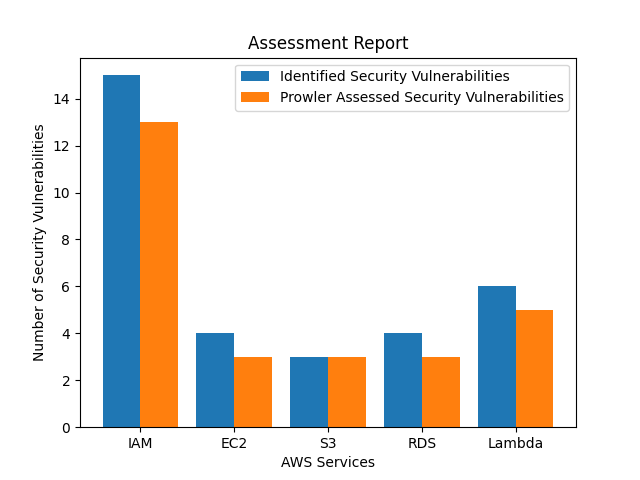
\includegraphics[width=\textwidth]{assessmentgraph.png}
    \caption{Prowler Assessment Graph}
    \label{fig:prowlerefficiency}
\end{figure}

\par The test-driven approach requires developing the test cases for the possible assessable scenario of a check in Prowler that performs the security assessment of an identified security vulnerability in the AWS service.
The individual test cases are developed, and their results are noted.

\par The checks in Prowler corresponding to the identified security vulnerabilities are identified manually.
The functionality of the check is understood and verified if the check can perform the assessment of the identified security vulnerability.
The verification process includes developing test cases for all assessable scenarios and evaluating the result of the assessment.
Only if all the scenarios are successfully verified the security vulnerability is marked to be assessed using Prowler.
Once all the test scenarios for the different checks in Prowler are developed and verified, the efficiency of Prowler is calculated against the identified security vulnerabilities for individual AWS services.
The efficiency calculation is done programmatically.

\begin{longtable}{|p{10cm}|p{2.4cm}|p{2cm}|}
    \hline
    \textbf{Security Vulnerabilities} & \textbf{Service} & \textbf{Prowler Check}\\
    \hline
    Avoid using root user account & IAM & Check11 \\
    \hline
    All IAM users have MFA enabled & IAM & Check12 \\
    \hline
    Disable unused credentials & IAM & Check13 \\
    \hline
    Access key rotation & IAM & Check14 \\
    \hline
    Account password contains at least one uppercase letter & IAM & Check15 \\
    \hline
    Account password contains at least one lowercase letter & IAM & Check16 \\
    \hline
    Account password contains at least one symbol & IAM & Check17\\
    \hline
    Account password contains at least one number & IAM & Check18\\
    \hline
    Account passwords fulfill minimum password length
    criteria & IAM & Check19\\
    \hline
    Prevents password reuse & IAM & Check110\\
    \hline
    Expiry password after 90 days & IAM & Check111\\
    \hline
    Administrator reset for expired password account & IAM & \\
    \hline
    Enable users to change their own account password & IAM& \\
    \hline
    Insider Threat & IAM & Extra774\\
    \hline
    Verify if root account has an access key & IAM &
    Check112 \\
    \hline
    Malicious AMI used to create EC2 instances & EC2 & Check76\\
    \hline
    User data public exposure & EC2 & Extra741\\
    \hline
    Server-Side Request Forgery & EC2 & Extra786\\
    \hline
    Denial of Wallet & EC2, Lambda &\\
    \hline
    S3 buckets publicly exposed & S3 & Check73\\
    \hline
    S3 buckets unencrypted & S3 & Extra764\\
    \hline
    S3 bucket public write access (GhostWriter) & S3 & Extra771 \\
    \hline
    RDS instances publicly accessible & RDS & Check78\\
    \hline
    RDS instances publicly accessible unencrypted & RDS & Extra735\\
    \hline
    Resources running in an AWS classic resource & RDS & \\
    \hline
    Default data retention for AWS RDS & RDS & Extra739\\
    \hline
    Lambda functions have a public resource-based policy & Lambda & Extra798 \\
    \hline
    AWS account publicly accessible & Lambda & Extra7145 \\
    \hline
    Public lambda function URL & Lambda & Extra7179 \\
    \hline
    Public lambda function URL Cors & Lambda & Extra7180 \\
    \hline
    Insecure Management of Secrets & Lambda & Extra760\\
    \hline
    Poisoning the Well & Lambda & \\
    \hline
    \caption{Prowler Checks and mapped Security Vulnerabilities}
    \label{tab:securityvulnerabilitiescheckin prowler}
\end{longtable}

\par The process for calculating the efficiency of Prowler begins by determining the count of the security vulnerabilities that are identified for an AWS service.
The table \ref{tab:classificationofsecurityvulnerabilities} shows all the security vulnerabilities that are identified in the five AWS services.
Additionally, the table also highlights the different checks in Prowler that are identified and verified by developing the test cases that assess these identified security vulnerabilities.
The count of number of security vulnerabilities that are identified for the AWS service is determined.
Also, the number of security vulnerabilities that are assessed using Prowler for that AWS service is determined.
Based on these results the efficiency of Prowler is calculated in assessing an AWS service.
For example, looking at the table \ref{tab:classificationofsecurityvulnerabilities} and the graph \ref{fig:prowlerefficiency} considering AWS RDS, the number of identified security vulnerabilities is 4, and the number of security vulnerabilities that are assessed using Prowler is 3.
This process is performed for the 5 AWS services that are chosen for this research work.
In the end, it is possible to determine how efficient Prowler is in assessing the security vulnerabilities of each AWS service.


\par The graph \ref{fig:prowlerefficiency} is drawn between the AWS services considered for this thesis work and the number of security vulnerabilities.
It highlights the total number of security vulnerabilities identified for an AWS service and the number of security vulnerabilities that are assessed using Prowler for the AWS service.

\par Looking at the graph for IAM, it can be concluded that out of the 15 identified security vulnerabilities, Prowler performs the assessment of 13 security vulnerabilities.
The 2 security vulnerabilities that cannot be assessed by
Prowler are \textit{Password expiration requires
administrator reset} and \textit{Enabling account users
to set new password}.
These security vulnerabilities are caused due to excessive privilege.
The Password expiration requires an administrator reset feature prevents the user from updating their password after the account password has expired and thus requires administrative access.
This causes an issue on the user’s productivity and increases the workload on the administrator but ensures account safety.
If the account user is given administrative permission, this avoids the impact on the user’s productivity, but at the same time increases the risk that the user can cause.
This user can reset passwords for another user, revoke or grant unrestricted access to resources, files or directories and can even delete other user resources or accounts.
By enabling this feature all the users to reset their
own account password.
If the user is granted an administrative role, the user would not just be able to change the password for his own account but would be able to manage other user accounts as well.
Assigning excessive privilege to a user can lead to 
deadly sin such as siphoning important information to the
competitors, data destruction, etc. \cite{89}.

\par Like IAM, looking at the graph for EC2 it can be determined that out of the 4 identified security vulnerabilities, 3 of those security vulnerabilities are assessed using Prowler.
 The unassessed security vulnerability using Prowler is the Denial of wallet.
 Most of the time data loss incidents make the news, but the denial of wallet is one of the common ways that can be found out about a compromise through the AWS bill.
 The denial of wallet security vulnerability causes 
disruption of the target system or flooding the system 
with traffic as a form of threat, ransom, or revenge thus
depriving the system usage or leading to downtime 
resulting in loss of time and money, and reputation
\cite{90}.

\par Prowler shows 100 \% efficiency in assessing the security vulnerabilities that are identified in S3 and thus Prowler is highly efficient in performing the security best practices assessments, audits, and incident response for S3.

\par Similar to IAM and EC2, out of 4 identified security
vulnerabilities prowler performs the assessment of 3 security vulnerabilities.
Prowler does not perform the assessment of security vulnerability that can occur due to RDS instances running on AWS classic resources.
The EC2-Classic platform is retired by Amazon and disabled on all accounts.
The EC2-Classic platform is replaced the EC2-VPC \cite{91}.

\par As seen from the graph \ref{fig:prowlerefficiency}, out of the 6 security vulnerabilities identified in AWS lambda, Prowler can perform the assessment of 5 security vulnerabilities.
The security vulnerability that is not assessed using Prowler is ‘Poisoning of well’.
Poisoning of well can be highly hazardous in numerous ways.
It can occur when the malicious users inject fake
training
data with the aim of corrupting the learned model and can
spread, affecting the products that draw from it or when
an \gls{ide} plugin
hosting the cloud server is controlled by an attacker.
A code backdoor is introduced as the security
vulnerability by the attacker into the plugin \cite{72}.


\section{Using Open-Source Application}

\begin{figure}
    \centering
    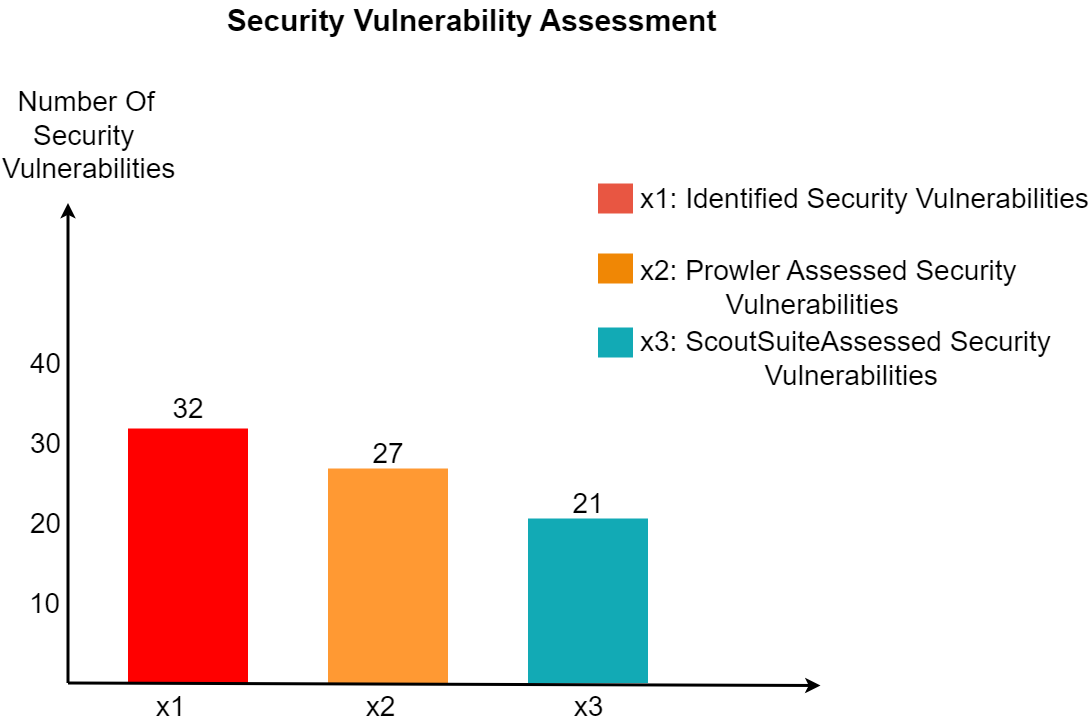
\includegraphics[width=\textwidth]{prowlervsscoutsuite.png}
    \caption{Security Vulnerabilities Assessment Graph}
    \label{fig:prowlervsscoutsuite}
\end{figure}

\par \gls{csp} make tools available to secure the cloud
systems,
but it is ultimately the user’s responsibility to use them.
The control needed to define and implement the cloud infrastructure differs greatly from the controls used in on-premises environments.
Simply transforming the hardware servers to AWS EC2 instances won't make the infrastructure secure by default.
This is because, while AWS is responsible for the
security of the cloud, it is the users responsibility
for the security in the cloud.
This resulted in organizations suffering from poorly
architected and misconfigured cloud infrastructure
leading to embarrassing data leaks \cite{92}.
This section shows the assessment of security vulnerability performed using two open-source cloud security assessment tools namely Prowler and ScoutSuite which can help strengthen the cloud security posture without breaking the bank.

\par The employee management web application \cite{78}
leverages different AWS services namely IAM, EC2, S3, RDS, and Lambda for its deployment on AWS cloud infrastructure as shown in the figure \ref{fig:infrastructure_architecture}.
Once the application is deployed on the AWS cloud, the application functionality is verified.
The application provides different functions such as adding, updating and deleting the organization’s employee information.
As the application deployment takes place, there could be a chance of introduction of security vulnerability due to misconfiguration or security flaws within the application.
In order to deal with these issues, the AWS account must be assessed using the assessment tools against any security vulnerability that might have been introduced while deploying the application on the AWS infrastructure.

\par To assess the AWS account against any security vulnerabilities two security assessment tools namely Prowler and ScoutSuite were introduced in chapter 4.

\par The assessment of AWS account against security vulnerabilities using Prowler is started via the command line by executing the command \textit{./prowler}.
After the assessment AWS account finishes, the assessment report is generated.
Prowler supports the generation of assessment reports in
multiple formats such as text, CSV, JSON, JSON-ASFF, JUnit-XML, and HTML. The generated assessment report provides a detailed description of the security vulnerability assessed, check in Prowler that assesses the security vulnerability, the result of the assessment, region, associated AWS service, etc. \cite{49}.


\par Similarly, the assessment using ScoutSuite is
started via the command line by executing the command
\textit{scout aws}.
When the assessment
of the AWS account finishes, the assessment report is generated in PDF format.
The assessment report provides a descriptive view of the 
different AWS services, the resources leveraged by each 
service, the rules available for each service, etc.
\cite{88}.


\par A total of 32 security vulnerabilities are identified in five AWS services based on literatures, the Open Web Application Security Project (OWASP) vulnerability list \cite{51}, Cybersecurity \& Infrastructure Security Agency (CISA) \cite{52}, International Data Corporation (IDC) \cite{53} as shown in the table \ref{tab:securityvulnerabilitiesandresources}.
After the assessment of the AWS account finishes, the following observation were determined:
\begin{itemize}
    \item Prowler was able to perform the assessment of 27 security vulnerabilities out of the 32 identified security vulnerabilities.
    There were 5 security vulnerabilities that could not be assessed using Prowler, as Prowler does not provide checks to assess those 5 security vulnerabilities.
\end{itemize}
\begin{itemize}
    \item ScoutSuite on the other hand performed the assessment of 21 security vulnerabilities successfully.
    There were 11 security vulnerabilities for which
    there were no rules provided by ScoutSuite.
\end{itemize}

\par The graph \ref{fig:prowlervsscoutsuite} shows the number of security vulnerabilities that were assessed by both the security assessment tools with regard to the total number of security vulnerabilities that were identified.

\begin{longtable}{|p{9cm}|p{4.2cm}|}
    \hline
    \textbf{Security Vulnerabilities} & \textbf{Identification Resource}\\
    \hline
    Insider threat & Literature \cite{93} \\
    \hline
    Misconfiguration: & OWASP \cite{51}, CISA \cite{52}, IDC \cite{53} \\
    \hline
    Instances created from Malicious AMI & Literature \cite{58} \\
    \hline
    User data public exposure & OWASP \cite{51} \\
    \hline
    Server-Side Request Forgery & OWASP \cite{51} \\
    \hline
    Denial of Wallet & CISA \cite{52} \\
    \hline
    Public exposure of S3 buckets & OWASP \cite{51}, Literature
    \cite{94}\\
    \hline
    Unencrypted S3 buckets & Literature \cite{95}\\
    \hline
    GhostWriter & CISA \cite{52} \\
    \hline
    Public RDS Database instance & OWASP \cite{51} \\
    \hline
    Resources running in AWS classic resources &
    Literature \cite{96}\\
    \hline
    Default data retention & Literature \cite{97} \\
    \hline
    Data Event Injection & OWASP \cite{51} \\
    \hline
    Insecure Management of Secrets & CISA \cite{52} \\
    \hline
    Poisoning the Well & CISA \cite{52} \\
    \hline
    \caption{Identified Security vulnerabilities}
    \label{tab:securityvulnerabilitiesandresources}
\end{longtable}

\par Based on the number of security vulnerabilities assessed, the efficiency of each tool can be evaluated.
To calculate the efficiency of each tool, the standard mathematical formula that evaluated the ratio of the output to input is used.
This formula expresses the result as a percentage \cite{98}.

\[ efficiency = (X/Y) * 100\]
\[  X: Number of security vulnerabilities assessed \]

\[  Y: Number of security vulnerabilities identified \]

Using this formula, the overall percentage efficiency of Prowler is calculated to be 84 \% and the overall efficiency of ScoutSuite is calculated to be 65 \%.

\par From the evaluated result for the two open-source security assessment tools can be inferred that Prowler possesses more checks than other tools miss.
It is a highly reliable and light piece of software with considerable documentation that helps developers and security auditors quickly set up and start security assessments.

\section{Comparision between Prowler and ScoutSuite}

\par In the previous sections of this chapter, the analysis was more manual.
In the first approach, the test cases were developed for the different checks in Prowler and the efficiency was evaluated.
In the second approach, an open-source application was
deployed
on the AWS infrastructure.
After the application
was deployed on AWS infrastructure, the assessment of
security vulnerabilities was performed.
Based on the result of the assessment the efficiency was calculated.
\\
\par In this section, a real-world situation is considered.
An organization plans to migrate from its on-premises data center setup to the AWS cloud infrastructure.
Migration involves moving all the organization’s workload, data, and applications to the AWS cloud.
During the migration process, different AWS services were
used such as RDS, EC2, etc.
\\
\par After the migration of the organization’s workload to the cloud finishes, the organization plans to use the cloud infrastructure to improve its customer experience.
But before starting to use the cloud infrastructure, the Security Engineers in the organization plan to perform a complete scan of the cloud infrastructure to avoid any security vulnerabilities that would have been introduced during the migration activity.
\\
\par To begin this process, the cloud administrator creates a user account called \textit{audit-user}.
The audit-user is used to audit AWS cloud infrastructure.
During this process, the cloud infrastructure is assessed to identify any security vulnerability that would have been introduced while migrating the organization’s workloads to the cloud.
The cloud administrator plans to provide limited privileges to the audit-user to perform the assessment and verify different AWS services.
The table \ref{tab:accountconfiguration} shows the list
of policies assigned to the audit-user.
\\
\begin{longtable}{|p{6cm}|p{8cm}|}
    \hline
    \textbf{AWS Service} & \textbf{Managed Policy}\\
    \hline
    EC2 & AmazonEC2ReadOnlyAccess \\
    \hline
    S3 & AmazonS3FullAccess \\
    \hline
    Lambda & AWSLambdaBasicExecutionRole,
    AWSLambdaReadOnlyAccess \\
    \hline
    RDS & AmazonRDSReadOnlyAccess \\
    \hline
    \caption{AWS account configuration}
    \label{tab:accountconfiguration}
\end{longtable}



\par Once the audit-user account is provisioned with the
required permission, the organization decides to
use Prowler and ScoutSuite as the assessment tools to perform the assessment of the organization’s cloud infrastructure.
To perform the assessment using Prowler and ScoutSuite additional managed policies namely \textit{SecurityAudit} and \textit{ViewOnlyAccess} are assigned to the audit-user.

\par The audit-user reviews the account and identifies a misconfiguration that would have been introduced while the audit-user account was configured.
The audit-user account was granted \textit{AmazonS3FullAccess} to the S3 bucket instead of read-only permission.
Assigning full access to the S3 bucket for the audit-user account led to the deviation from the least privilege principle.
It grants the user full access to the S3 buckets.
Taking advantage of this permission, the user can change the block public access setting, disable encryption of the bucket, and perform several other hazardous operations on the S3 buckets using this permission.

\par After reviewing the account, the audit-user starts the assessment of the cloud infrastructure using the two tools.
The audit-user configures the AWS cloud environment with the credentials and starts the assessment by running the commands \textit{./prowler} and \textit{scout aws} to perform the assessment using Prowler and scout aws respectively.

\par Once the assessment of the cloud infrastructure using
the two tools finishes, the assessment reports were generated.
Upon analyzing the assessment report several security vulnerabilities in the cloud infrastructure were identified.

\par The organization leverages two S3 buckets for storing the application files.
One of the S3 buckets during the assessment was found to be publicly accessible.
Additionally, it was found that both buckets were not encrypted and did not have bucket logging enabled.

\par The organization data and information were stored in AWS RDS. The RDS instance was configured on a single availability zone.
Hence in case of loss of availability, the failover to another instance would not possible.

\par The infrastructure had a lambda function.
This lambda function had a policy attached to it that allowed access to any AWS account.


\par In addition to identifying the above security
vulnerabilities, the AWS account was assessed against the
security
vulnerabilities identified for this research work.
The table \ref{tab:comparisionresultprowlervsscoutsuite}
below lists the different the security
vulnerabilities that were assessed using each tool
individually.

\begin{longtable}{|p{8cm}|p{2.4cm}|p{2cm}|p{2cm}|}
    \hline
    \textbf{Security Vulnerabilities} & \textbf{Service} & \textbf{Prowler} & \textbf{ScoutSuite}\\
    \hline
    Avoid using root user account & IAM & {{\color{green}\checkmark}} & {{\color{green}\checkmark}} \\
    \hline
    All IAM users have MFA enabled & IAM & {{\color{green}\checkmark}} & {{\color{green}\checkmark}}\\
    \hline
    Disable unused credentials & IAM & {{\color{green}\checkmark}} & {{\color{green}\checkmark}}\\
    \hline
    Access key rotation & IAM & {{\color{green}\checkmark}} & {{\color{green}\checkmark}}\\
    \hline
    Account password contains at least one uppercase letter & IAM & {{\color{green}\checkmark}} & {{\color{green}\checkmark}}\\
    \hline
    Account password contains at least one lowercase letter & IAM & {{\color{green}\checkmark}} & {{\color{green}\checkmark}}\\
    \hline
    Account password contains at least one symbol & IAM & {{\color{green}\checkmark}} & {{\color{green}\checkmark}}\\
    \hline
    Account password contains at least one number & IAM & {{\color{green}\checkmark}} & {{\color{green}\checkmark}}\\
    \hline
    Account password fulfill minimum password length criteria & IAM & {{\color{green}\checkmark}} & {{\color{green}\checkmark}}\\
    \hline
    Prevents password reuse & IAM & {{\color{green}\checkmark}} & {{\color{green}\checkmark}}\\
    \hline
    Expiry password after 90 days & IAM & {{\color{green}\checkmark}} & {{\color{green}\checkmark}}\\
    \hline
    Administrator reset for expired password account & IAM &  &\\
    \hline
    Enable users to change their own account password & IAM & &\\
    \hline
    Insider Threat & IAM & {{\color{green}\checkmark}} & {{\color{green}\checkmark}}\\
    \hline
    Verify if root accounthas an access key & IAM & {{\color{green}\checkmark}} & {{\color{green}\checkmark}}\\
    \hline
    Malicious AMI used to create EC2 instances & EC2 & {{\color{green}\checkmark}} & {{\color{green}\checkmark}}\\
    \hline
    User data public exposure & EC2 & {{\color{green}\checkmark}} & {{\color{green}\checkmark}}\\
    \hline
    Server-Side Request Forgery & EC2 & {{\color{green}\checkmark}} & \\
    \hline
    Denial of Wallet & EC2, Lambda & &\\
    \hline
    S3 buckets publicly exposed & S3 &  {{\color{green}\checkmark}} & {{\color{green}\checkmark}}\\
    \hline
    S3 buckets uneccrypted & S3 & {{\color{green}\checkmark}} & {{\color{green}\checkmark}}\\
    \hline
    S3 bucket public write access (GhostWriter) & S3 & {{\color{green}\checkmark}} & {{\color{green}\checkmark}}\\
    \hline
    RDS instances publicly accessible & RDS & {{\color{green}\checkmark}} & {{\color{green}\checkmark}}\\
    \hline
    RDS Instance unencrypted & RDS & {{\color{green}\checkmark}} & {{\color{green}\checkmark}}\\
    \hline
    Resources running in an AWS classic resource & RDS & &\\
    \hline
    Default data retention for AWS RDS & RDS & {{\color{green}\checkmark}} & {{\color{green}\checkmark}}\\
    \hline
    Lambda functions have a public resource-based policy & Lambda & {{\color{green}\checkmark}} & \\
    \hline
    AWS account publicly accessible & Lambda & {{\color{green}\checkmark}} & \\
    \hline
    Public lambda function URL & Lambda & {{\color{green}\checkmark}} &\\
    \hline
    Public lambda function URL Cors & Lambda & {{\color{green}\checkmark}} & \\
    \hline
    Insecure Management of Secrets & Lambda & {{\color{green}\checkmark}} &\\
    \hline
    Poisoning the Well & Lambda & & \\
    \hline
    \caption{Prowler vs ScoutSuite security vulnerability assessment}
    \label{tab:comparisionresultprowlervsscoutsuite}
\end{longtable}


\par Looking at the assessment results in the table \ref{tab:comparisionresultprowlervsscoutsuite}, it
is possible to determine how efficient individual security
tools
are in performing the security assessment of the security vulnerabilities associated with the different AWS services.

\par Starting with IAM, it can be inferred that both Prowler and ScoutSuite are equally efficient in performing the assessment of identified security vulnerabilities.
The two security vulnerabilities that were left unassessed by both tools occurs due to excessive privilege issue.
There are no checks in Prowler, and there are no rules in ScoutSuite to perform the security assessment of those security vulnerabilities.

\par For EC2, it can be seen that Prowler does not
contain a check to assess Denial of Wallet security
vulnerability, on the other hand, there are no rules in
ScoutSuite to assess Server-Side Request Forgery and
Denial of Wallet security vulnerabilities.

\par The table shows that both tools were able to perform
the assessment of all the identified security vulnerabilities in S3 and thus no security vulnerability is left unassessed.

\par Based on the assessment report for RDS, it is seen that both the tools cannot perform the assessment of the RDS instance running on AWS classic resource.

\par ScoutSuite does not provide rules to access AWS
Lambda \cite{86}, thus assessing the Lambda function is
not possible using ScoutSuite.
From the table
\ref{tab:comparisionresultprowlervsscoutsuite}, it can be
seen that Poisoning of Well is not assessed using Prowler.